\documentclass[12pt, A4]{article}

% Packages
	% Basics
		\usepackage{amsmath}
		\usepackage{bm}
		\usepackage{cellspace}
		\usepackage{csquotes}
		\usepackage{fixltx2e}
		\usepackage[hang,flushmargin]{footmisc}
		\usepackage[margin=0.5in]{geometry}
		\usepackage{hyperref}
		\usepackage[utf8]{inputenc}
		\usepackage{mathtools}
		\usepackage{multirow}
	% Diagrams
		\usepackage{pgfplots}
		\usepackage{tikz}
			\usepackage{circuitikz} % Circuits
			\usepackage{tikz-3dplot} % 3D
			\usetikzlibrary{arrows.meta, angles, calc, quotes}
	% Notation
		\usepackage{amssymb} % Miscellaneous
		\usepackage{chemformula} % Chemical Formulas
		\usepackage{esint} % Integrals
		\usepackage{mathrsfs} % Laplace
		\usepackage{physics} % Differentials/Vectors
		\usepackage{siunitx} % Units

% Macros
	% Notation
		% Constants
			\newcommand{\en}{\text{e}}
		% Functions
			\DeclareMathOperator{\erfc}{erfc}
			\DeclareMathOperator{\Uscr}{\mathscr{U}}
		% Sets
			\newcommand{\N}{\mathbb{N}}
			\newcommand{\R}{\mathbb{R}}
			\newcommand{\Z}{\mathbb{Z}}
		% Transforms
			\DeclareMathOperator{\Ell}{\mathscr{L}}
			\DeclareMathAlphabet{\mathscrbf}{OMS}{mdugm}{b}{n}
		% Other
			\DeclareMathOperator{\avg}{avg}
			\renewcommand{\Roman}[1]{\MakeUppercase{\romannumeral #1}}
			\renewcommand{\th}{\text{th}}
	% Utilities
		\newcommand{\callout}[2]{\begin{center}\fbox{\begin{minipage}{#1cm}#2\end{minipage}}\end{center}}
		\newcommand{\comment}[1]{}
		\newcommand{\subsectionb}[1]{\subsection*{#1}\addcontentsline{toc}{subsection}{#1}}
		\newcommand{\subsubsectionb}[1]{\subsubsection*{#1}\addcontentsline{toc}{subsubsection}{#1}}
		\newcommand{\subt}[2]{#1_{\text{#2}}}
		\newcommand{\supt}[2]{#1^{\text{#2}}}
		
% Configuration
	\title{Differential Equations Cheat Sheet}
	\author{Arnav Patri and Shashank Chidige}
	\date{}
	\hypersetup{
	    colorlinks,
	    citecolor=black,
	    filecolor=black,
	    linkcolor=black,
	    urlcolor=black
	}
	\cellspacetoplimit10pt
	\cellspacebottomlimit10pt
	
\begin{document}
	\maketitle
	\tableofcontents
	\setcounter{section}{-1}
	\section{Preliminary Information}
		\begin{align*}
			\sinh x &= \frac{\en^x - \en^{-x}}{2} &
				\cosh x &= \frac{\en^x + \en^{-x}}{2} \\
			\sinh(-x) &= -\sinh(x) &
				\cosh(-x) &= \cosh(x) \\
			\cosh^2x - \sinh^2x &= 1 &
				2 - \tanh^2x &= \sech^x \\
			1 - \coth^2x &= -\csch^2 &
				\sinh(u + v) &= \sinh u \cosh v + \cosh x \sinh v \\
			\cosh(u + v) &= \cosh u \cosh v + \sinh u \sinh v
		\end{align*}
		\begin{verbatim}
			syms y(x)
			ode = diff(y, x, 2) - y == exp(3x)
			ySol(x) = dsolve(ode)
		\end{verbatim}
		\texttt{diff(y, x, n)} is the \(\supt{n}{th}\) derivative of \(y\) with respect to \(x\).
		\[\begin{array}{|c|*{5}{c}|}\hline
			f(x) & \ln x & \tan x & \cot x & \sec x & \csc x \\\hline
			\int f(x) \dd{x} & x(\ln x - 1) & \ln|\sec x| & \ln|\sin x| & \ln|\tan x + \sec x| & -\ln|\csc x - \cot x| \\\hline
		\end{array}\]
		\[\begin{array}{|c|*{6}{c}|}\hline
			f(x) & \sinh x & \cosh x & \tanh x & \sech x & \csch x & \coth x \\\hline
			f'(x) & \cosh x & \sinh x & \sech^2 x & -\sech x\tanh x & -\csch x \coth x & -\csch^2 x \\\hline
			\int f(x) \dd{x} &\cosh x & \sinh x & \ln(\cosh x) & \arctan(\sinh x) & -\ln|\csch x - \coth x| & \ln(\sinh|x|) \\\hline
		\end{array}\]
		\[\def\arraystretch{2}\begin{array}{|c|*{6}{c}|}\hline
			f(x) & \arcsin x & -\arccos x & \arctan x & -\arccot x & \arcsec x & -\arccsc x \\\hline
			f'(x) & \multicolumn{2}{c}{\dfrac{1}{\sqrt{1 - x^2}}} & \multicolumn{2}{c}{\dfrac{1}{1 + x^2}} & \multicolumn{2}{c|}{\dfrac{1}{|x|\sqrt{x^2 - 1}}} \\\hline
		\end{array}\]



	\section{Introduction to Differential Equations}
		A \textbf{differential equation (DE)} is a function relating one or more unknown functions (dependent variables) to one or more independent variables. \\
		A differential equation with a \textit{single} independent variable is said to be an \textbf{ordinary differential equation (ODE)}. One with \textit{more than one} is said to be a \textbf{partial differential equation (PDE)}. \\
		An ODE is \textbf{linear} if the dependent variable and all of its derivatives are raised only to the first power; that is, it can be written as
			\[a_n(x)\dv[n]{y}{x} + a_{n - 1}(x)\dv[n - 1]{y}{x} + \cdots + a_1(x)\dv{y}{x} + a_0(x)y = g(x)\]
			It is \textbf{nonlinear} if it is not linear. \\
		An \textbf{\(\bm{\supt{n}{th}}\)-order} ODE is one where the highest derivative of the dependent variable is its \(\supt{n}{th}\) derivative. \\
		A first-order linear DE in \textbf{differential form} is 
			\[M(x, y)\dd{x} + N(x, y)\dd{y} = 0\]
		A DE is in \textbf{normal form} if it can be written as
			\[\dv[n]{y}{x} = f\left(x, y, y', \ldots, y^{(n)}\right)\]
			where \(f\) is a real-valued function. \\
		An \(\supt{n}{th}\)-order \textbf{initial value problem (IVP)} is a set of values, called \textbf{initial conditions}, that \(x\), \(y\), and its first \(n - 1\) derivatives must be equal to at a single point. If conditions are set at multiple points, called \textbf{boundary conditions}, it is a \textbf{boundary-value problem (BVP)}.
	\section{First-Order Differential Equations}
		\subsection{Separable Equations}
			A first-order ODE is separable if it is of the form
				\[\dv{y}{x} = g(x)h(y)\]
				Rewriting and integrating, the DE can be solved as
				\[\int \frac{\dd{y}}{h(y)} = \int g(x)\dd{x}\]
		\subsection{The Integrating Factor}
			\comment{
				Consider the first-order linear DE
					\[a_1(x)\dv{y}{x} + a_0(x)y = g(x)\]
					This can be rewritten in standard form as
					\[\dv{y}{x} + P(x)y = f(x)\]
					where \(P(x) + a_0(x)/a_1(x)\) and \(f(x) = g(x)/a_1(x)\).
					The \textbf{integrating factor \(\bm{\mu(x)}\)} is found as
					\[\mu(x) = \en^{\int P(x)\dd{x}}\]
					Multiplying by this on both sides yields
					\begin{align*}
						\en^{\int P(x)\dd{x}}f(x) &= \en^{\int P(x)\dd{x}}\dv{y}{x} + P(x)\en^{\int P(x)\dd{x}}y \\
							&= \dv{x}\left[\en^{\int P(x) \dd{x}}\right]
					\end{align*}
					which is separable. Integrating on both sides yields
					\[
						\en^{\int P(x)\dd{x}}y = \int \en^{\int P(x) \dd{x}}f(x)\dd{x} + C
					\]
					This is a one-parameter family of solutions
					\[y = \en^{-\int P(x)\dd{x}}\int \en^{\int P(x)}f(x) \dd{x} + C\en^{-\int P(x)}\]
					In summary, to solve a linear first-order DE,
			}
			\callout{12}{\paragraph{Solving a Linear First-Order Differential Equation}
				\begin{enumerate}
					\item 
						Put the DE into standard form
							\[\dv{y}{x} + P(x)y = f(x)\]
					\item
						Identify \(P(x)\) and find the \textbf{integrating factor \(\bm{\mu(x)}\)} as
							\[\mu(x) = \en^{\int P(x) \dd{x}}\]
					\item
						Multiply by \(\mu(x)\) on both sides, yielding 
						\[\dv{x}\left[y\en^{\int P(x) \dd{x}}\right] = \en^{\int P(x)\dd{x}}f(x)\]
					\item
						Integrate on both sides and solve for \(y\)
				\end{enumerate}
				}
		\subsection{Exact Equations}
			The \textbf{differential} of a function \(z = f(x, y)\) is
				\[\dd{z} = \pdv{z}{x} + \pdv{z}{y}\]
				In the special case that \(f(x, y) = 0\), this is 0. 
				A differential equation
				\[M(x, y)\dd{x} + N(x, y)\dd{y} = 0\]
				is an \textbf{exact equation} if the left-side is an \textbf{exact differential}, which is true if
				\[\pdv{M}{y} = \pdv{N}{x}\]
				The solution to the DE can then be found as
				\begin{align*}
					f(x, y) &= \int M(x, y) \dd{x} + g(y) \\
						&= \int N(x, y) \dd{y} + g(x)
				\end{align*}
				In the first case,
				\[
					\pdv{f}{y} = N(x, y)
						= \dv{y}\int M(x, y) \dd{x} + g'(y)
				\]
				\(g'(y)\) can then be solved for an integrated to derive \(g(y)\) and \(f(x, y)\). A similar method works for the second case. \\
				The solution of the DE is
				\[C = f(x, y)\]
				Consider a first-order DE in differential form that is not exact; that is,
				\[\pdv{M}{y} \ne \pdv{N}{x}\]
				It can be made exact by multiplying by the integrating factor \(\mu(x)\), or \(\mu(y)\), found as
				\[
					\mu(x) = \en^{\int \frac{M_y - N_x}{N}\dd{x}} \qquad \text{and} \qquad
					\mu(y) = \en^{\int \frac{N_x - M_y}{M}\dd{y}}
				\]
				It is not guaranteed that either will exist in terms of a single variable, so both must be tested.
		\subsection{Substitutions}
			A function \(f(x, y)\) is homogenous if
				\[f(tx, ty) = t^\alpha f(x, y)\]
				for some real number \(\alpha\), called the degree. A first-order DE in differential form
				\[M(x, y)\dd{x} + N(x, y)\dd{y} = 0\]
				is said to be homogenous if both \(M\) and \(N\) are homogenous and of the same degre. If both are homogenous, then it can be written that
				\[\begin{array}{ccccc}
					\begin{aligned}
						M(x, y) &= x^\alpha M(1, u) \\
						M(x, y) &= y^\alpha M(v, 1)
					\end{aligned} & \text{and} &
					\begin{aligned}
						N(x, y) &= x^\alpha N(1, u) \\
						N(x, y) &= y^\alpha M(v, 1)
					\end{aligned} & \text{where} &
					\begin{aligned}
						u &= \frac{y}{x} \\
						v &= \frac{x}{y}	
					\end{aligned}
				\end{array}\]
				Product rule can be used to solve for the differential that now lacks a variable. \\
				\begin{align*}
					\dd{y} &= x\dd{u} + u\dd{x} &
						\dd{x} &= y\dd{u} + u\dd{y}	
				\end{align*}
				Substituting this and \(M\) and \(N\) in terms of the new variable back into the equation makes it separable, allowing it to be solved. \\
			\textbf{Bernoulli's equation} is 
				\[\dv{y}{x} + P(x)y = f(x)y^n\]
				where \(n\) is a real number. The substitution \(u = y^{1 - n}\) reduces this equation to a linear equation.
	\setcounter{section}{3}
	\section{Higher-Order Differential Equations}
		\subsection{Superposition}
			A linear \(\supt{n}{th}\)-order DE of the form
				\[a_n(x)\dv[n]{y}{x} + a_{n - 1}(x)\dv[n - 1]{y}{x} + \cdots + a_1(x)\dv{y}{x} + a_0(x)y = 0\]
				is said to be \textbf{homogenous} while one of the form
				\[a_n(x)\dv[n]{y}{x} + a_{n - 1}(x)\dv[n - 1]{y}{x} + \cdots + a_1(x)\dv{y}{x} + a_0(x)y = g(x)\]
				where \(g(x)\) is not identically 0 is said to be \textbf{nonhomogenous}. \\
				The \textbf{associated homogenous equation} of a nonhomogenous DE is the nonhomogenous DE minus \(g(x)\). \\
			\(D\) is a \textbf{differential operator} defined by
				\[D^ny = \dv[n]{y}{x}\]
				An \textbf{\(\bm{\supt{n}{th}}\)-order differential operator} or \textbf{polynomial operator \(\bm{L}\)} is defined as
				\[L = a_n(x)D^n + a_{n - 1}(x)D^{n - 1} + \cdots + a_1(x)D + a_0(x)\]
				It should be noted that \(D\) and \(L\) are \textbf{linear operators}; that is, 
				\[L\{\alpha f(x) + \beta g(x)\} = \alpha L(f(x)) + \beta L(g(x))\]
				A linear homogenous equation and a nonhomogenous equation can be written respectively as
				\[
					L(y) = 0 \qquad \text{and} \qquad
					L(y) = g(x)
				\]
			The \textbf{superposition} of functions is a linear combination of them. If \(y_{i\cdots k}\) are solutions to \(L(y) = 0\), then, the general solution can be written as
				\[y = c_1y_1(x) + c_2y_2(x) + \cdots + c_ky_k(x)\]
				where the \(c_i\) are arbitrary constants.
			A set of functions \(f_1(x), f_x(x), \ldots, f_n(x)\) is said to be \textbf{linearly dependent} on an interval \(I\) if there exist constants \(c_i\) (that are not all 0) such that
				\[c_1f_1(x) + c_2f_2(x) + \cdots + c_nf_n(x) = 0\]
				for every \(x\) in the interval. If a set of functions are not linearly dependent on an interval, they are \textbf{linearly independent}.
			Let each of the functions \(f_1(x), f_2(x), \ldots, f_n(x)\) possess at least \(n - 1\) derivatives. The determinant
				\[
					W(f_1, f_2, \ldots, f_n) = \begin{vmatrix}f_1 & f_2 & \cdots & f_n \\ f_1' & f_2' & \cdots & f_n' \\ \vdots & \vdots && \vdots \\ f_1^{(n - 1)} & f_2^{(n - 1)} & \cdots & f_n^{(n - 1)}\end{vmatrix}
				\]
				is the \textbf{Wronskian} of the functions. \\
			Let \(y_1, y_2, \ldots, y_n\) be \(n\) solutions of the homogenous linear \(n^{\th}\)-order DE \(L(y) = 0\) on interval \(I\). The set of solutions is \textbf{linearly independent} on \(I\) if an only if \(W(y_1, y_2, \ldots, y_n) \not\equiv 0\) for every \(x\) in the interval. \\
			Any set of \(n\) linearly independent solutions of the homogenous linear \(n^{\th}\)-order linear DE \(L(y) = 0\) on an interval \(I\) is said to be a \textbf{fundamental set of solutions} on the interval. \\
			The solution of a nonhomogenous DE is the sum of the \textbf{complementary solution \(\bm{y_c}\)}, the solution to the associated homogenous equation, and the \textbf{particular solution \(y_p\)} that is free of parameters; that is,
				\[y = y_c + y_p\]
		\subsection{Reduction of Order}
			Consider the homogenous linear second-order DE
				\[a_2(x)y''+ a_1(x)y' + a_0(x)y = 0\]
				This can be put into standard form by dividing by \(a_2(x)\):
				\[y'' + P(x)y' + Q(x)y = 0\]
				Given a solution \(y_1\), a second solution \(y_2\) can be found as
				\[\boxed{y_2 = y_1\int \frac{\en^{-\int P(x) \dd{x}}}{y_1^2}\dd{x}}\]
		\subsection{Homogenous Equations with Constant Coefficients}
			Consider the homogenous linear second-order DE
				\[ay'' + by' + cy = 0\]
				with constant coefficients \(a\), \(b\), and \(c\). Assume that the solution is of the form \(y = \en^{mx}\). Substituting this yields
				\begin{align*}
					0 &= am^2\en^{mx} + bm\en^{mx} + c\en^{mx} \\
						&= (am^2 + bm + c)\en^{mx}
				\end{align*}
				\(\en^{mx}\) is never equal to 0, so
				\[\boxed{am^2 + bm + c = 0}\]
				This is the \textbf{auxiliary equation} of the DE. If the roots are two distinct real numbers \(m_1\) and \(m_2\), the solution is
				\[y = C_1\en^{m_1x} + C_2\en^{m_2x}\]
				If there is only a single real root \(m_1\),
				\[y = \en^{m_1x}(C_1 + C_2m)\]
				If there are 2 distinct imaginary roots \(m_2\) and \(m_2\),
				\[y = C_1\cos(m_1 x) + C_2\cos(m_2 x)\]
				This logic also applies to higher-order equations.
		\subsection{Undetermined Coefficients}
			\subsubsection{Superposition Approach}
				The form of \(y_p\) for a nonhomogenous linear DE can be found from that of \(g(x)\):
					\callout{17}{\paragraph{Trial Particular Solutions}
						\[\def\arraystretch{1.3}\begin{array}{|c|c|}\hline
							g(x) & \text{Form of } y_p \\\hline
							k & A \\
							ax^n + bx^{n - 1} + \cdots & Ax^n + Bx^{n - 1} + \cdots \\
							\sin(\alpha x) & \multirow{2}*{\(A\cos(\alpha x) + B\sin(\alpha x)\)} \\
							\cos(\alpha x) & \\
							\en^{kx} & A\en^{kx} \\\hline
						\end{array}\]
						The form of \(y_p\) when \(g(x)\) is the product of two functions is that of one function with the second function's substituted in for the constants. If \(g(x) = (ax + b)\sin x\), for example, then \(y_p = (Ax + B)\cos x + (Cx + E)\sin x\). When \(g(x)\) is a sum, the form is simply the sum of the forms of the individual terms of \(g(x)\).
					}
					If one of the \(y_p\) contains terms that are duplicated in \(y_c\), those terms must be multiplied by \(x^n\), where \(n\) is the smallest positive integer that avoids duplication.
			\subsubsection{Annihilator Approach}
				An \textbf{annihilator operator} of \(f(x)\) is an operator that makes \(f(x)\) 0.
					\[\begin{array}{|c|ccccc|}\hline
						f(x) & k & x^m & x^m\en^{\alpha x} & x^m\en^{\alpha x}\cos(\beta a) & x^m\en^{\alpha x}\sin(\beta x) \\\hline
						L & D & D^{m + 1} & (D - \alpha)^{m + 1} & \multicolumn{2}{c|}{\left[D^2 - 2\alpha D + \left(\alpha^2 + \beta^2\right)\right]^{m + 1}} \\\hline
					\end{array}\]
					Applying the annihilator operator for \(g(x)\) to both sides of a nonhomogenous DE yields the form of \(y_p\).
		\subsection{Variation of Parameters}
			Let \(y_1\) be a known solution of
				\[\dv{y_1}{x} + P(x)y_1 = 0\]
				It is clear that
				\[y_1 = C\en^{-\int P(x)\dd{x}}\]
				is the general solution.
				\textbf{Variation of parameters} involves finding a solution of a corresponding nonhomogenous equation
				\[\dv{y}{x} + P(x)y = g(x)\]
				that is of the form
				\[y_p = u_1(x)y_1(x)\]
				replacing the \textit{parameter} \(C\) with a \textit{function} \(u_1\). this into the DE yields
				\begin{align*}
					f(x) &= \dv{x}[u_1y_1] + P(x)u_1y_1 \\
						&= u_1\dv{y_1}{x} + y_1\dv{u_1}{x} + P(x)u_1y_1 \\
						&= u_1\left[\dv{y_1}{x} + P(x)y_1\right] + y_1\dv{u_1}{x} \\
						&= y_1\dv{u_1}{x}
				\end{align*}
				Separating variables yields
				\[\dd{u_1} = \frac{f(x)}{y_1(x)}\dd{x}\]
				Integrating,
				\[u_1 = \int \frac{f(x)}{y_1(x)}\dd{x}\]
				making the particular solution
				\[y_p = y_1\int \frac{f(x)}{y_1(x)}\dd{x}\]
			Consider the standard-form nonhomogenous linear second-order DE
				\[y'' + P(x)y' + Q(x)y = f(x)\]
				The complementary solution is
				\[y_c = C_1y_1(x) + C_2y_2(x)\]
				so the desired particular solution is of the form
				\[y_p = u_1(x)y_1(x) + u_2(x)y_2(x)\]
				Substituting this into the DE yields the system
				\begin{align*}
					y_1u_1' + y_2u_2' &= 0 &
						y_1'u_1' + y_2'u_2' &= f(x)	
				\end{align*}
				the solution of which can be expressed in terms of the determinants
				\begin{align*}
					u_1' &= \frac{W_1}{W} = -\frac{y_2f(x)}{W} &
						u_2' &= \frac{W_2}{W} = \frac{y_1f(x)}{W}	
				\end{align*}
				where \(W\) is the Wronskian of \(y_1\) and \(y_2\) and \(W_i\) is \(W\) with the \(\supt{i}{th}\) column replaced by 0's until the bottom-most element, which is \(f(x)\). \\
				For an \(\supt{n}{th}\)-order linear nonhomogenous DE,
					\[u_i' = \frac{W_i}{W}\]
		\subsection{Cauchy-Euler Equations}
			A \textbf{Cauchy-Euler equation} is of the form
				\[a_nx^n\dv[n]{y}{x} + a_{n - 1}x^{n - 1}\dv[n - 1]{y}{x} + \cdots + a_1x\dv{y}{x} + a_0y = g(x)\]
				Assume a solution \(y = x^m\). Each term becomes a polynomial in \(n\), as
				\[
					a_kx^k\dv[k]{y}{x} 
						= a_kx^km(m - 1)(m - 2)\cdots(m - k + 1)x^{m - k} 
						= a_km(m - 1)(m - 2)\cdots(m - k + 1)x^m
				\]
				Factoring the result of the substitution for a homogenous second-order Cauchy-Euler equation yeilds
				\[
					ax^2\dv[2]{y}{x} + bx\dv{y}{x} + cy
						= am(m - 1)x^m + bmx^m + cx^m
						= (am(m - 1) + bm + c)x^m
				\]
				The \textbf{auxiliary equation} is then
				\[\boxed{
					0 = am(m - 1) + bm + c = a^2 + (b - a)m + c
				}\]
				If this equation has distinct real roots \(m_1\) and \(m_2\), the solution is
				\[y = C_1x^{m_1} + C_2x^{m_2}\]
				If it has repeated real root \(m_1\), the solution is
				\[y = C_1x^{m_1} + C_2x^{m_1}\ln x\]
				If it has distinct imaginary roots \(m_1\) and \(m_2\), the solution is
				\[y = x^\alpha[C_1\cos(\beta\ln x) + C_2\sin(\beta\ln x)]\]
			The method of constant coefficients does not carry over to nonhomogenous DEs with variable coefficients \textit{in general}. Variation of parameters can instead be employed. \\
			Any Cauchy-Euler equation can be rewritten as a linear DE with constant coefficient by means of the substitution \(x = e^t\). Once a general solution to the DE in terms of \(t\) is found, the substitution \(t = \ln x\) can be made to find the solution in terms of \(x\). \\
			To solve a Cauchy-Euler equation for \(x < 0\), the substitution \(t = -x\) can be made. Using chain rule,
				\[
					\dv{y}{x} = \dv{y}{t}\dv{t}{x} = -\dv{y}{t} \qquad \text{and} \qquad
					\dv[2]{y}{x} = \dv{t}\left(-\dv{y}{t}\right)\dv{t}{x} = \dv[2]{y}{t}
				\]
			A second-order DE of the form
				\[a(x - x_0)^2\dv[2]{y}{x} + b(x - x_0)\dv{y}{x} + cy = 0\]
				is also a Cauchy-Euler equation. This can be solved by seeking a solution of the form \(y = (x - x_0)^m\), using the substitutions
				\[
					\dv{y}{x} = m(x - x_0)^{m - 1} \qquad \text{and} \qquad
						\dv[2]{y}{x} = m(m - 1)(x - x_0)^{m - 2}
				\]
				Alternatively, the DE can be reduces by the substitution \(t = x - x_0\) and solved normally before resubstituting.
		\subsection{Green's Functions}
			If \(y_1\) and \(y_2\) form a fundamental set of solutions to the homogenous form of
				\[y'' + P(x)y' + Q(x)y = f(x)\]
				variation of parameters shows that
				\[y_p(x) = y_1(x)\int_{x_0}^x \frac{-y_2(t)f(t)}{W(t)}\dd{t} + y_2(x)\int_{x_0}^x \frac{y_1(t)f(t)}{W(t)}\dd{t}\]
				for an IVP with conditions at \(x_0\). This can be rewritten as
				\[\boxed{y_p(x) = \int_{x_0}^x G(x, t)f(t)\dd{t}}\]
				where
				\[\boxed{G(x, t) = \frac{y_1(t)y_2(x) - y_1(x)y_2(t)}{W(t)}}\]
				is the \textbf{Green's function} of the IVP. \\
				The solution to the IVP
					\[y'' + P(x)y' + Q(x)y = f(x), \quad y(x_0) = y_0, y'(x_0) = y_1\]
					is
					\[y = y_h + y_p\]
					where \(y_p\) is as defined above and \(y(h)\) is the solution of
					\[y'' + P(x)y' + Q(x)y = 0, \quad y(x_0) = y_0, y'(x_0) = y_1\]
			Consider the a second-order linear nonhomogenous BVP with conditions at \(a\) and \(b\). The coefficient functions can be found to be
				\[
					u_1(x) = -\int_b^x\frac{y(t)f(t)}{W(t)}\dd{t} \qquad \text{and} \qquad
					u_2(x) = \int_a^x\frac{y_1(t)f(t)}{W(t)}\dd{t}
				\]
				This final solution can be compactly written as the single integral
				\[\boxed{y_p(x) = \int_a^b G(x, t)f(t) \dd{t}}\]
				where
				\[\boxed{
					G(x, t) = \begin{cases}
						\dfrac{y_1(t)y_2(x)}{W(t)} & a \le t \le x \\
						\dfrac{y_1(x)y_2(t)}{W(t)} & x \le t \le b
					\end{cases}
				}\]
				is the \textbf{Green's function} of the BVP.
		\subsection{Systems of Linear DEs}
			A DE can be written by rewriting in terms of differential operators:
				\[
					a_ny^{(n)} + a_{n - 1}y^{(n - 1)} + \cdots + a_1y' + a_0y = g(t)
						= \left(a_nD^n + a_{n - 1}D^{n - 1} + \cdots + a_1D + a_0\right)y 
				\]
				A system of DEs can be solved via rewriting in terms of these differential operators and solving via elimination.
		\subsection{Nonlinear DEs}
			When the dependent variable is missing from a DE, the substitution \(u = y'\) can be made:
				\[
					0 = F(x, y', y'') 
						= F(x, u, u')
				\]
				This equation can then be solved for \(u\) and the result integrated for \(y\). \\
			When the independent variable is missing from a DE, the same substitution can be made:
				\[
					0 = F(y, y', y'')
						= F\left(y, u, u\dv{u}{y}\right)
				\]
	\section{Modeling with Higher-Order Differential Equations}
		\subsection{Springs}
			Hooke's law states that the \textbf{spring force \(\bm{F_s}\)} (the force applied by a spring on a body towards equilibrium) is proportional to the displacement of the spring from equilibrium (the amount of elongation) \(s\). The constant of proportionality \(k\) is the \textbf{spring constant} and is a property of the spring.
				\[F = -ks\]
			Newton's second law states that force \(F\) is the product of the mass \(m\) and acceleration \(a\) of the body.
				\[F = ma\]
				The acceleration due to gravity is \(g \approx 9.8\) \(\mathrm{m/s^2}\), so the force due to gravity \(F_s\) or weight \(W\) is
					\[F_g = W = mg\]
				Acceleration is simply the second derivative of position, so
				\[
					m\dv[2]{x}{s} =
						F_g - F_s
						= mg - k(x + s)
						= mg - kx - ks
				\]
				\textit{Note that gravity is in the positive direction, so down is positive and up is negative}. \\ 
				If \(s\) is the spring's equilibrium position, the spring is not moving, which means that the \(F_s\) and \(F_g\) cancel, so \(mg = ks\):
				\[m\dv[2]{x}{t} = -kx\]
			\subsubsection{Free Undamped Motion}
				Dividing by \(m\) yeilds the DE of \textbf{free undamped motion} or \textbf{simple harmonic motion}
					\[\dv[2]{x}{t} + \omega^2x = 0\]
					where \(\omega^2 = k/m\). The auxiliary equation is evidently
					\[m^2 + \omega^2 = 0\]
					This has two imaginary solutions \(m_{1,2} = \pm i\omega\), making the equation of motion
					\[x(t) = C_1\cos(\omega t) + C_2\sin(\omega t)\]
					The \textbf{period of motion \(\bm{T}\)} (in s) is
					\[T = \frac{2\pi}{\omega}\]
					and the \textbf{frequency \(\bm{f}\)} (in hz or \(\mathrm{s^{-1}}\)) is simply its reciprocal
					\[
						f = \frac{1}{T}
							= \frac{\omega}{2\pi}
					\]
				\(\omega\) (in rad/s) is sometimes referred to as the \textbf{natural frequency} of the system. \\
				The \textbf{amplitude of free vibrations \(\bm{A}\)} is
					\[A = \sqrt{C_1^2 + C_2^2}\]
					It is often convenient to rewrite the equation of motion as
					\[x(t) = A\sin(\omega t + \varphi)\]
					where \(\varphi\) is the \textbf{phase angle} defined by
					\[
						\left.\begin{aligned}
							\sin\varphi &= \frac{C_1}{A} \\
							\cos\varphi &= \frac{C_2}{A}
						\end{aligned}\right\}
						\tan\varphi = \frac{C_1}{C_2}
					\]
					A cosine function is sometimes preferred, making the solution
					\[x(t) = A\cos(\omega t + \varphi)\]
					where \(\varphi\) is defined by
					\[
						\left.\begin{aligned}
							\sin\varphi &= \frac{C_2}{A} \\
							\cos\varphi &= \frac{C_1}{A}
						\end{aligned}\right\}
						\tan\varphi = \frac{C_2}{C_1}
					\]
					In reality, it is reasonable to expect the spring constant to decay over time. One model for the \textbf{aging spring} replaces the spring constant \(k\) with the decreasing function
					\[K(t) = k\en^{-\alpha t}\]
					where \(k\) and \(\alpha\) are positive constants. The linear DE
					\[mx'' + k\en^{-\alpha t}x = 0\]
					cannot be solved with the methods discussed thus far. \\
					When a spring/mass system is subject to a rapidly decreasing temperature, \(k\) may be replaced with \(K(t) = kt\) where \(k\) is a positive constant, a function that increases with time. The resulting model
					\[mx'' + ktx = 0\]
					is a form of \textbf{Airy's differential equation}.
			\subsubsection{Free Damped Motion}
				Damping forces are those that gradually decay the acceleration of the body. It is assumed that the damping force is a constant multiple of velocity. Adding this term to the second law formulation yields
					\[m\dv[2]{x}{t} = -k - \beta\dv{x}{t}\]
					where \(\beta\) is a positive \textbf{damping constant}. Dividing by \(m\) and rewriting yields
					\[0 = \dv[2]{x}{t} + 2\lambda \dv{x}{t} + \omega^2 x\]
					where \(\omega^2 = k/m\) and \(2\lambda = \beta/m\). The auxiliary equation is then
					\[0 = m^2 + 2\lambda m + \omega^2\]
					which has roots
					\[m_{1, 2} = -\lambda \pm \sqrt{\lambda^2 - \omega^2}\]
				If the discriminant is greater than 0 (\(\lambda > \omega\)), the situation is said to be \textbf{overdamped}, and the solution is
					\[x(t) = \en^{-\lambda t}\left(C_1\en^{t\sqrt{\lambda^2 - \omega^2}} + C_2\en^{-t\sqrt{\lambda^2 - \omega^2}}\right)\]
					If the discriminant is 0 (\(\lambda = \omega\)), the system is said to be \textbf{critically damped}, and the solution is
					\[x(t) = \en^{-\lambda t}\left(C_1 + C_2t\right)\]
					If the discriminant is less than 0 (\(\lambda < \omega)\), the system is said to be \textbf{underdamped}, and the solution is
					\[x(t) = \en^{-\lambda t}\left(C_1\cos(t\sqrt{\omega^2 - \lambda^2}) + C_2\sin(t\sqrt{\omega^2 - \lambda^2})\right)\]
				Any solution
					\[x(t) = \en^{-\lambda t}\left(C_1\cos\left(t\sqrt{\omega^2 - \lambda^2}\right) + C_2\sin\left(t\sqrt{\omega^2 - \lambda^2}\right)\right)\]
					can be rewritten as
					\[x(t) = A\en^{-\lambda t}\sin\left(t\sqrt{\omega^2 - \lambda^2} + \varphi\right)\]
					where
					\[
						A = \sqrt{C_1^2 + C_2^2} \qquad \text{and} \qquad
						\tan\varphi = \frac{C_1}{C_2}
					\]
					\(A\en^{-\lambda t}\) is sometimes referred to as the \textbf{damped amplitude} of vibrations. \\
				As the solution is not periodic, the number
					\[\frac{2\pi}{\sqrt{\omega^2 - \lambda^2}}\]	
					is called the \textbf{quasi period} and
					\[\frac{\sqrt{\omega^2 - \lambda^2}}{2\pi}\]
					the \textbf{quasi frequency}. \\
					The quasi period is the interval between two successive maxima.
		\subsection{Eigenvalues and Eigenfunctions}
			Many problems require the solving of a 2-point BVP involving a linear DE containing a parameter \(\lambda\). \textit{Nontrivial (nonzero)} solutions are sought. \\
			Consider the BVP
				\[
					y'' + \lambda y = 0, \quad
					y(0) = 0, \quad
					y(L) = 0
				\]
			For \(\lambda = 0\), the solution of \(y'' = 0\) is \(y = C_1x + C_2\). The conditions imply that \(C_1 = C_2 = 0\), so the only solution is the trivial solution \(y = 0\). The same applies to \(\lambda < 0\). \\
			For \(\lambda > 0\), it is convenient to write \(\lambda = -\alpha^2\) (where \(\alpha \in \R^+\)). The roots of the auxiliary equation \(m^2 + \alpha^2 = 0\) are then \(m = \pm i\alpha\), so the general solution of
				\[y'' + \alpha^2y = 0\]
				is
				\[y = C_1\cos(\alpha x) + C_2\sin(\alpha x)\]
				\(y(0)\) again implies that \(C_1  0\) and the condition \(y(L) = 0\) or
				\[C_2\sin(\alpha L) = 0\]
				is satisfied by \(C_2 = 0\). This again yields the trivial solution \(y = 0\). If it is required that \(C_2 \ne 0\), though, then \(\sin(\alpha L) = 0\) is satisfied so long as \(\alpha L\) is an integer multiple of \(\pi\):
				\[
					\alpha L = n\pi \quad \text{or} \quad
					\alpha = \frac{n\pi}{L} \quad \text{or} \quad
					\lambda_n = \alpha_n^2 = \left(\frac{n\pi}{L}\right)^2, \quad
					n \in \Z^+
				\]
				For any real nonzero \(C_2\),
				\[y_n(x) = C_2\sin\left(\frac{n\pi x}{L}\right)\]
				is a solution for \(n \in \Z^+\). As the DE is homogenous, any constant multiple of a solution is itself also a solution, so \(C_2\) can be set to 1. In other words, for each number in the sequence
				\[\lambda_n = \frac{n^2\pi^2}{L^2} \quad \text{for} \quad n \in \Z^+\]
				the corresponding function
				\[y_n = \sin\left(\frac{n\pi}{L}\right)\]
				is a nontrivial solution of the problem
				\[
					y'' + \lambda_ny = 0, \quad
					y(0) = 0, \quad
					y(L) = 0
				\]
				The numbers \(\lambda_n\) are known as \textbf{eigenvalues}. The nontrivial solutions are called \textbf{eigenfunctions}.
	\section{Series Solutions of Linear Equations}
		\subsection{Power Series}
			A \textbf{power series centered at \(\bm{a}\)} is an infinite series of the form
				\[\sum_{n = 0}^\infty c_n(x - a)^n\]
			\subsubsection{Convergence}
				A power series is \textbf{convergent} at a value of \(x\) if its sequence of partial sums \(\{\{S_N(x)\}\}\) converges; that is,
					\[\lim_{N \to \infty}S_N(x) = \lim_{N \to \infty}\sum_{n = 0}^Nc_n(x - a)^n\]
					must exist. If this limit does not exist, the series is said to be \textbf{divergent}. \\
				 The \textbf{interval of convergence} is the set of \textit{all} real numbers \(x\) for which the series converges. Every power series has one. \\
				 The radius \(R\) of the interval of convergence is the \textbf{radius of convergence}. If \(R > 0\), then a power series converges for \(|x - a| < R\) (equivalently \(a - R < x < a\)  and diverges for \(|x - a| > R\). If the series is only convergent at its center, \(R = 0\). If it converges for all \(x \in \R\), then \(R = \infty\). It may or may not converge at the endpoints of the interval. \\
				 The power series \textbf{converges absolutely} within its interval of convergence (not inclusive), meaning that
				 	\[\sum_{n = 0}^\infty\left|c_n(x - a)^n\right|\]
				 	converges. \\
				 The convergence of a power series can often be determined by the \textbf{ratio test}. If \(c_n \ne 0\) for all \(n \in \N\), let
				 	\[
				 		\lim_{n \to \infty}\left|\frac{c_{n + 1}(x - a)^{n + 1}}{c_n(x - a)^n}\right|
				 			= |x - a|\lim_{n \to \infty}\left|\frac{c_{n + 1}}{c_n}\right|
				 			= L
					\]
					If \(L < 1\), the series converges absolutely. If \(L > 1\), it diverges. If \(L = 1\), the test is inconclusive. This test is always inconclusive at the endpoints of the interval of convergence.
			\subsubsection{A Power Series Defines a Function}
				A power series defines a function
						\[f(x) = \sum_{n = 0}^\infty c_n(x - a)^n\]
						whose domain is the the series' interval of convergence. If the radius of convergence is \(R > 0\), the \(f\) is continuous, differentiable, and integrable on \(a \pm R\). If it is \(\infty\), \(f\) is continuous, differentiable, and integrable on \(\R\). \(f'(x)\) and \(\int f(x)\dd{x}\) can be found term-by-term via differentiation or integration. Convergence at the endpoints may be gained through integration or lost through differentiation. \\
					If
						\[y = \sum_{n = 0}^\infty c_nx^n\]
						is a power series, then
						\[
							y' = \sum_{n = 0}^\infty c_nnx^{n - 1} \qquad \text{and} \qquad
							y'' = \sum_{n = 0}^\infty c_nn(n - 1)x^{n - 2}
						\]
						It is then clear that the first term of \(y'\) and the first 2 of \(y''\) are 0. Omitting these, they become
						\[
							y' = \sum_{n = 1}^\infty c_nnx^{n - 1} \qquad \text{and} \qquad
							y'' = \sum_{n = 2}^\infty c_nn(n - 1)x^{n - 2}
						\]
						Note in particular the changed lower bound of the summation in the derivatives.
			\subsubsection{Properties}
				The \textbf{identity property} states that if
					\[\sum_{n = 0}^\infty c_n(x - a)^n = 0\]
					and \(R > 0\), then \(c_n = 0\) for all \(n \in \N\). \\
				A function \(f\) is said to be \textbf{analytic at a point} if it can be represented at that point with a power series with a radius of convergence that is either positive or infinite. \\
				Power series may be combined through addition, multiplication, and division. \\
				Two power series can be added by shifting the summation indices such that the degree of \(x\) is the same for both and then taking any terms out of one power series to make the lower bound the same.
				\callout{17}{\paragraph{Common Maclaurin Series}
					\[\def\arraystretch{2}\begin{array}{|c|c|c|}\hline
						f(x) & \text{Maclaurin Series} & \text{Interval of Convergence} \\\hline
						e^x & \displaystyle\sum_{n = 0}^\infty \frac{1}{n!}x^n & \R \\
						\cos x & \displaystyle\sum_{n = 0}^\infty \frac{(-1)^n}{(2n)!}x^{2n} & \R \\
						\sin x & \displaystyle\sum_{n = 0}^\infty \frac{(-1)^n}{(2n + 1)!}x^{2n + 1} & \R \\
						\arctan x & \displaystyle\sum_{n = 0}^\infty \frac{(-1)^n}{2n + 1}x^{2n + 1} & [-1, 1] \\
						\cosh x & \displaystyle\sum_{n = 0}^\infty \frac{1}{(2n)!}x^{2n} & \R \\
						\sinh x & \displaystyle\sum_{n = 0}^\infty \frac{1}{(2n + 1)!}x^{2n + 1} & \R \\
						\ln(1 + x) & \displaystyle\sum_{n = 1}^\infty \frac{(-1)^{n + 1}}{n}x^n & (-1, 1] \\
						\displaystyle\frac{1}{1 - x} & \displaystyle\sum_{n = 0}^\infty x^n & (-1, 1) \\\hline
					\end{array}\]
				}
		\subsection{Solutions}
			A point \(x = x_0\) is said to be an \textbf{ordinary point} of the DE
				\[a_2(x)y'' + a_1(x)y' + a_0(x)y = 0\]
				if both \(P(x)\) and \(Q(x)\) are analytic at \(x_0\), where
				\[y'' + P(x)y' + Q(x)y = 0\]
				is the standard form of the DE. A point that is not an ordinary point of this DE is a \textbf{singular point} of it. \\
			The coefficients functions considered are typically polynomials, making \(P(x)\) and \(Q(x)\) rational functions, which are analytic everywhere apart from where their denominators. It then follows that \textit{A number \(x = x_0\) is an ordinary point of the DE if \(a_2(x_0) \ne 0\). Otherwise it is a singular point.}
			\subsubsection{About Ordinary Points}
				If \(x = x_0\) is an ordinary point of
					\[a_2(x)y'' + a_1(x)y' + a_0(x)y = 0\]
					then 2 linearly independent solutions of the form
					\[y = \sum_{n = 0}^\infty c_n(x - x_0)^n\]
					can always be found. \\
				A power series solution converges on at least some interval defined by \(|x - x_0| < R\), where \(R\) is the distance between \(x_0\) and the closest singular point, called the \textit{minimum value} or \textit{lower bound} of the radius of convergence. \\
				A solution of the above form is a \textbf{solution about the ordinary point \(\bm{x_0}\)}. \\
				The power series solution about the ordinary point \(x = 0\)
				\[\boxed{y = \sum_{n = 0}^\infty c_nx^n} \]
				and its first 2 derivatives are
				\[\boxed{
					y' = \sum_{n = 1}^\infty nc_nx^{n - 1} \qquad \text{and} \qquad
					y'' = \sum_{n = 2}^\infty n(n - 1)c_nx^{n - 2}
				}\]
				Substituting these into the DE and rewriting in terms of a single power series enables a recurrence relation to be found for \(c_n\). Letting the initial coefficients be 1 allows for a non-recursive equation for \(c_n\) to be found.
			\subsubsection{About Singular Points}
				A singular point \(x = x_0\) is said to be a \textbf{regular point} of
					\[a_2(x)y'' + a_1(x)y' + a_0(x)y = 0\]
					if 
					\[
						p(x) = (x - x_0)P(x) \qquad \text{and} \qquad
						q(x) = (x - x_0)^2Q(x)
					\]
					where
					\[
						P(x) = \frac{a_1(x)}{a_2(x)} \qquad \text{and} \qquad
						Q(x) = \frac{a_0(x)}{a_2(x)}
					\]
					are both analytic at \(x_0\). One that is not regular is \textbf{irregular}. \\
					\textit{If \(x - x_0\) appears at most to the \(\supt{1}{st}\) power in the denominator of \(P(x)\) and at most to the \(\supt{2}{nd}\) power in that of \(Q(x)\), then \(x = x_0\) is a regular singular point.}
				\callout{17}{\paragraph{Frobenius' Theorem}
				If \(x = x_0\) is a regular singular point of a second-order homogenous linear DE, then there exists \textit{at least} one solution of the form
					\[
						y = (x - x_0)^r\sum_{n = 0}^\infty c_n(x - x_0)^n
							= \sum_{n = 0}^\infty c_n(x - x_0)^{n + r}
					\]
					where \(r\) is a constant. The series converges at least on some interval \(0 < x - x_0 < R\).
				}
				The \textbf{method of Frobenius} involves substituting
					\[y = \sum_{n = 0}^\infty c_n(x - x_0)^{n + r}\]
					into the DE to derive a recurrence relation for \(c_n\). Before determining the coefficient, though, \(r\) must be determined. \\
				The \textbf{indicial equation} is found by substituting the power series solution into the DE and simplifying, yielding a quadratic equation in \(r\) that results from equating the \textit{total coefficient of the lowest power of \(x\) to 0}. Solving for the values of \(r\) and substituting these into the a recurrence relation allows at least one solution of the assumed form to be found. If \(r \notin \N\), then the corresonding solution is not a power series.\\
				The general indicial equation for
					\[a_2(x)y'' + a_1(x)y' + a_0(x)y = 0\]
					can be found to be
					\[\boxed{0 = r(r - 1) + a_0r + b_0}\]
					where \(a_0\) and \(b_0\) are the first (the constant) terms of the power series of \(p(x)\) and \(q(x)\) respectively. \\
				If the roots of the indicial equation are 2 distinct real numbers \(r_1\) and \(r_2\) with \(r_1 > r_2\) and \(r_1 - r_2 \notin \Z^+\), then there exist 2 linearly independent solutions of the forms
					\[
						y_1(x) = \sum_{n = 0}^\infty c_nx^{n + r_1}, \quad c_0 \ne 0 \qquad \text{and} \qquad 
						y_2(x) = \sum_{n = 0}^\infty b_nx^{n + r_2}, \quad b_0 \ne 0
					\]
					If the roots are distinct real numbers \(r_1\) and \(r_2\) with \(r_1 > r_2\) and \(r_1 - r_2 \in \Z\), there exist 2 linearly independent solutions of the forms
					\[
						y_1(x) = \sum_{n = 0}^\infty c_nx^{n + r_1}, \quad c_0 \ne 0 \qquad \text{and} \qquad
						y_2(x) = Cy_1(x)\ln x + \sum_{n = 0}^\infty b_nx^{n + r_2}, \quad b_0 \ne 0
					\]
					where \(C\) is a (potentially 0) constant. \\
					If the only a single root \(r_1\) exists, there always exist 2 linearly independent solutions of the forms
					\[
						y_1(x) = \sum_{n = 0}^\infty c_nx^{n + r_1}, \quad c_0 \ne 0 \qquad \text{and} \qquad
						y_2(x) = y_1(x)\ln x + \sum_{n = 1}^\infty b_nx^{n + r_1}
					\]
				When \(r _1 - r_2 \in \Z^+\) (the second case described above), there \textit{may} be 2 solutions of the form
					\[y = \sum_{n = 0}^\infty c_nx^{n + r}\]
					This is cannot be known in advance, instead being determined after finding the indicial roots and examining the recurrence relation that defines the coefficients \(c_n\). It is possible that \(C = 0\); that is,
					\[
						y_1(x) = \sum_{n = 0}^\infty c_nx^{n + r_1} \qquad \text{and} \qquad
						y_2(x) = \sum_{n = 0}^\infty b_nx^{n + r_2}
					\]
					When only a single solution exists (the third case described above), the method of Frobenius fails to provide a second series solution; the second solution always contains a logarithm. A second solution with the logarithmic term can be obtained by using the fact that
					\[y_2(x) = y_1(x) \int\frac{\en^{-\int P(x)\dd{x}}}{y_1^2(x)}\dd{x}\]
					is also a solution of the DE when \(y_1(x)\) is a known solution.
	\section{The Laplace Transform}
		An \textbf{integral transform} is defined as
			\[\int_0^\infty K(s, t)f(t) \dd{t} = \lim_{b \to \infty}\int_0^b K(s, t)f(t) \dd{t}\]
			where \(K(s, t)\) is called the \textbf{Kernel} of the transform. The kernel of the \textbf{Laplace transform \(\mathscrbf{L}\)} is \(K(s, t) = \en^{-st}\), making it
				\[\Ell\{f(t)\} = \int_0^\infty \en^{-st}\dd{t} = F(s)\]
		\subsection{Properties}
			The Laplace transform is \textbf{linear}, meaning that
				\[\Ell\{\alpha f(x) + \beta g(x)\} = \alpha F(x) + \beta G(x)\]
				where \(\alpha\) and \(\beta\) are constants.
			\callout{14}{\paragraph{Transforms of Some Basic Functions}
				\[\def\arraystretch{3}\begin{array}{|c|*{7}{c}|}\hline
					f(t) & 1 & t^n & \en^{\alpha t} & \sin(kt) & \cos(kt) & \sinh(kt) & \cosh(kt) \\\hline
					\Ell\{f(t)\} & \dfrac{1}{s} & \dfrac{n!}{s^{n + 1}}, n \in \Z^+ & \dfrac{1}{s - a} & \dfrac{k}{s^2 + n^2} & \dfrac{s}{s^2 + k^2} & \dfrac{k}{s^2 - k^2} & \dfrac{s}{s^2 - k^2} \\\hline
				\end{array}\]
			}
		\subsection{Invers Transforms}
			If \(F(s) = \Ell\{f(t)\}\), \(f(t)\) is the \textbf{inverse Laplace transform} of \(F(s)\), denoted
				\[f(t) = \Ell^{-1}\{F(s)\}\]
			\callout{14}{\paragraph{Some Inverse Transforms}
				\[\def\arraystretch{3}\begin{array}{|c|*{7}{c}|}\hline
					F(s) & \dfrac{1}{s} & \dfrac{n!}{s^{n + 1}}, n \in \N & \dfrac{1}{s - a} & \dfrac{k}{s^2 + k^2} & \dfrac{s}{s^2 + k^2} & \dfrac{k}{s^2 - k^2} & \dfrac{s}{s^2 - k^2} \\\hline
					\Ell^{-1}\{F(s)\} & 1 & t^n & \en^{at} & \sin(kt) & \cos(kt) & \sinh(kt) & \cosh(kt) \\\hline
				\end{array}\]
			}
			Just like \(\Ell\), \(\Ell^{-1}\) is a linear transform. \\
			Decomposing a fraction into its partial fractions often aids in evaluating inverse transforms. \\
		\subsection{Derivative Transforms}
			If \(f'\) is continuous, integration by parts gives
				\[
					\Ell\{f'(t)\} = \int_0^\infty \en^{-st}f'(t)\dd{t}
						= \left[\en^{-st}f(t)\right]_0^\infty + s\int_0^\infty \en^{-st}f(t)
						= -f(0) + s\Ell\{f(t)\}
				\]
				or
				\[\Ell\{f'(t)\} = sF(s) - f(0)\]
				A similar process holds for higher-order derivatives.
			\callout{17}{\paragraph{Theorem 7.2.2 Transform of a Derivative}
				If \(f, f', \ldots, f^{(n - 1)}\) are continuous on \([0, \infty\) and of exponential order and if \(f^{(n)}(t)\) is piecewise continuous on \([0, \infty)\), then
					\[
						\Ell\left\{f^{(n)}\right\} = s^nF(s) - s^{n - 1}f(0) - s^{n - 2}f'(0) - \cdots - f^{(n - 1)}(0)
							= s^nF(s) - \sum_{i = 1}^n s^{n - i}f^{(i - 1)}(0)
					\]
					where \(F(s) = \Ell\{f(t)\}\).
			}
			The Laplace transform can be applied to both sides of a differential equation.
			\callout{9.03}{
				\textit{The Laplace transform of a linear DE with constant coefficients becomes an algebraic equation in \(Y(s)\).}
			}
			\callout{17}{\paragraph{Steps in solving an IVP by the Laplace transform}
				\[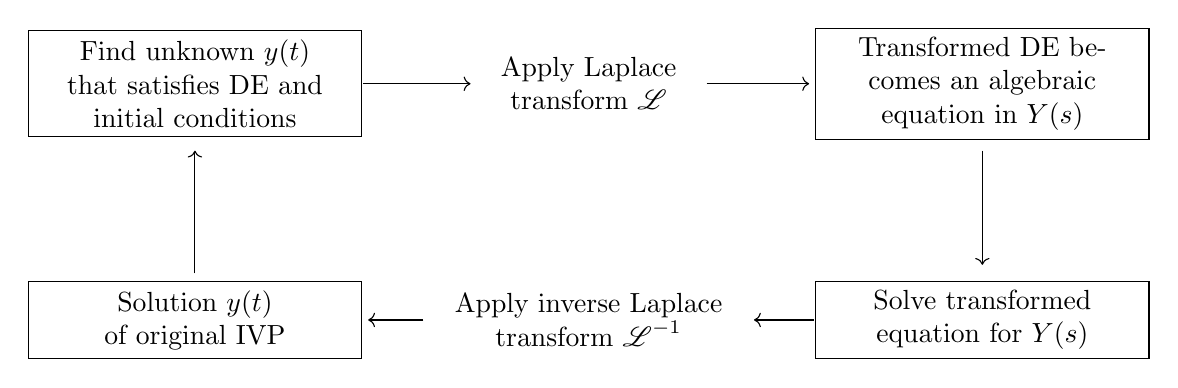
\begin{tikzpicture}
					\node at (-5, 1) [draw, align = center, text width = 4cm] {Find unknown \(y(t)\) that satisfies DE and initial conditions};
						\draw[->] (-2.86, 1) -- (-1.5, 1);
					\node at (0, 1) [align = center, text width = 4cm] {Apply Laplace transform \(\Ell\)};
						\draw[->] (1.5, 1) -- (2.8, 1);
					\node at (5, 1) [draw, align = center, text width = 4cm] {Transformed DE becomes an algebraic equation in \(Y(s)\)};
						\draw[->] (5, 0.15) -- (5, -1.3);
					\node at (5, -2) [draw, align = center, text width = 4cm] {Solve transformed equation for \(Y(s)\)};
						\draw[->] (2.86, -2) -- (2.1, -2);
					\node at (0, -2) [align = center, text width = 4cm] {Apply inverse Laplace transform \(\Ell^{-1}\)};
						\draw[->] (-2.1, -2) -- (-2.8, -2);
					\node at (-5, -2) [draw, align = center, text width = 4cm] {Solution \(y(t)\) of original IVP};
						\draw[->] (-5, -1.41) -- (-5, 0.15);
				\end{tikzpicture}\]
			}
		\subsection{Operational Properties}
			\callout{13.88}{\paragraph{Translation on the \(\bm{s}\)-axis}
					If \(\Ell\{f(t)\} = F(s)\) and \(a\) is a real number, then
						\[\Ell\{\en^{at}f(t)\} = F(s - a)\]
				}
			For emphasis, it is sometimes useful to use the notation
				\[\Ell\{\en^{at}f(t)\} = \Ell\{f(t)\}|_{s \to s - a}\]
				where \(s \to s - a\) means that the Laplace transform \(F(s)\) replaces \(s\) with \(s - a\) wherever it appears.
			To compute the inverse of \(F(s - a)\), \(F(s)\) must be recognized. \(\Ell^{-1}\{F(s - a)\}\) is then simply the product of \(f(t) = \Ell^{-1}F(s)\) and \(\en^{at}\). Symbolically, this can be summarized as
				\[
					\Ell^{-1}\{F(s - a)\} = \Ell^{-1}\{F(s)|_{s \to s - a}\}
						= \en^{at}f(t)
				\]
			\callout{17}{\paragraph{Unit Step Function}
				The \textbf{unit step function} (or \textbf{Heaveside function}) \(\Uscr(t - a)\) is defined to be
					\[
						\Uscr(t - a) =
							\begin{cases}
								0 & 0 \le t < a \\
								1 & t \ge a	
							\end{cases}
					\]
			}
			When a function \(f\) defined for \(t \ge 0\) is multiplied by \(\Uscr(t - a)\), the unit step function \enquote{turns off} the portion of the graph that is before \(t = a\). \\
			The unit step function can be used to compactly write piecewise functions:
				\[
					f(t) =
						\begin{cases}
							g(t) & 0 \le t < a \\
							h(t) & t \ge a	
						\end{cases}
						= g(t) - g(t)\Uscr(t - a) + h(t)\Uscr(t - a)
				\]
				\[
					f(t) = 
						\begin{cases}
						0 & 0 \le t < a \\
						g(t) & 	a \le t < b \\
						0 & t \ge b
						\end{cases}
						= g(t)[\Uscr(t - a) - \Uscr(t - b)]
				\]
		\callout{15.65}{\paragraph{Translation on the \(\bm{t}\)-axis}	
			If \(F(s) = \Ell\{f(t)\}\) and \(a > 0\), then
				\[\Ell\{f(t - a)\Uscr(t - a)\} = \en^{-as}F(s)\]
		}
		When \(a > 0\),
				\[\Ell^{-1}\{\en^{-as}F(s)\} = f(t - a)\Uscr(t - a)\]
		Using the definition of \(\Uscr(t - a)\) and the substitution \(u = t - a\), the transform of the product of a function and a step function can be rewritten as
				\[
					\Ell\{g(t)\Uscr(t - a)\} = \int_a^\infty \en^{-st}g(t)\dd{t}
						= \int_0^\infty \en^{-s(u + a)}g(u + a) \dd{u}
				\]
				That is,
				\[\boxed{\Ell\{g(t)\Uscr(t - a)\} = \en^{-as}\Ell\{g(t + a)\}}\]
		\callout{17}{\paragraph{Derivatives of Transforms}
			If \(F(s) = \Ell\{f(t)\}\) and \(n \in \Z^+\), then
				\[\Ell\{t^nf(t)\} = (-1)^n\dv[n]{s}F(s)\]
		}
		If \(f\) and \(g\) are piecewise continuous on the interval \([0, \infty)\), then their \textbf{convolution}, denoted by \(f * g\), is defined by
			\[f * g = \int_0^t f(\tau)g(t - \tau)\dd{\tau}\]
			This is a function of \(t\). As  such, this is sometimes written as \((f * g)(t)\). As the notation suggests, convolution can be interpreted as the \textit{generalized product} of two functions. It should be noted that this is commutative, so \(f * g = g * f\).
		\callout{17}{\paragraph{Convolution Theorem}
			If \(f(t)\) and \(g(t)\) are piecewise continuous on \([0, \infty)\) and of exponential order, then
				\[
					\Ell\{f * g\} = \Ell\{f(t)\}\Ell\{g(t)\}
						= F(s)G(s)
				\]
		}
		It is evident that
			\[\Ell\{F(s)G(s)\} = f * g\]
		When \(g(t) = 1\) and \(\Ell\{g(t)\} = G(s) = 1/s\), the convolution theorem implies that the Laplace transform of the integral of \(f\) is
			\[\Ell\left\{\int_0^t f(\tau) \dd{\tau}\right\} = \frac{F(s)}{s}\]
			The inverse form of this is
			\[\int_0^t f(\tau) \dd{\tau} = \Ell^{-1}\left\{\frac{F(s)}{s}\right\}\]
		The \textbf{Volterra integral equation} is
			\[f(t) = g(t) + \int_0^t f(\tau)h(t - \tau)\dd{\tau}\]
			where \(g(t)\) and \(h(t)\) are both known. This can be solved by taking the Laplace transform of both sides, as this can be rewritten as
			\[f(t) = g(t) + (f * h)(t)\]
			so
			\[F(s) = G(s) + F(s)H(s)\]
			This can then be solved for \(F(s)\), the inverse transform of which can be taken to find \(f(t)\).
\end{document}

